\documentclass[letterpaper, 12pt]{article}
\usepackage{graphicx} % Required for inserting images
\usepackage{textcomp}
\usepackage{fullpage}
\usepackage{amsmath}
\usepackage{xcolor}
\usepackage{float}
\usepackage{geometry}
\usepackage{biblatex}
\geometry{margin=1in}
\usepackage{enumitem}
\usepackage{microtype}
\usepackage{gensymb}
\usepackage{parskip}
\usepackage{tikz}
\usepackage{caption}
\usepackage{cancel}
\usepackage{nicefrac}


\usepackage{hyperref}
\hypersetup{
    colorlinks=true,        % Enable colored links
    linkcolor=teal,         % Set color for internal links
    citecolor=teal,         % Set color for citations
    filecolor=teal,         % Set color for file links
    urlcolor=teal           % Set color for URLs
}

\usepackage[version=4]{mhchem}

\title{Amino acids}
\author{BIOS 1006}
\date{18 June 2025}

\begin{document}

\maketitle

\section*{Objectives}

\begin{itemize}
\item Describe the properties of amino acids, in general
\item Learn the names, abbreviations, adjectives, functional groups (structures) and properties of all 20 common $\alpha$-amino acids
\item Identify the polar, hydrophobic, polar, acidic or basic features in amino acid structures, and predict how two amino acid R-groups can interact
\item Rationalize the position of each amino acid R-group on the hydropathy scale
\item Describe the spectroscopic properties of amino acids
\item Know the pKa values of the R-groups (do not need to memorize), the average amino group and the average carboxylic acid group
\item Determine the net charge of an amino acid or peptide at a specific pH
\item Calculate the pI values of amino acids and small peptides
\item Draw the chemical structures of amino acid functional groups at different pHs
\item Extract pKa values from titration data
\item Describe the importance of a protein’s pI in biological function
\item Describe the roles of amino acids in biological systems
\item Identify the amino acid from which amino acid derivatives are derived
\end{itemize}

\newpage

\section*{Definitions}

\newpage

\section*{Amino acids}

\subsection*{Roles of amino acids}

\begin{itemize}
\item Determine the structure of proteins
\item Provide basis for protein function
\item Signaling molecules
\item Precursors for other biomolecules
\item Intermediates in metabolic processes
\end{itemize}

\subsection*{Amino acid properties}
\begin{itemize}
\item Zwitterionic (both positive and negative charges) and amphoteric (both an acid and a base) at pH 7
\item Contains amino, hydrogen, carboxyl, and R-group (variant)
\item Average molecular weight: 110 kDa
\item $\alpha$ amino acids have 2 different stereoisomers (different arrangements) that are enantiomers (mirror images)
\item Classified as D or L (in biological systems, L isomer is most common)
\item Amino on the left = L, amino on the right = D
\item Stereochemistry makes a big difference!
\end{itemize}

\subsection*{The amino acids}

\subsubsection*{Functional groups found in amino acids}

\begin{itemize}
\item Alcohols
\item Thiols
\item Thioethers
\item Carboxylic acids
\item Amides
\item Basic groups
\end{itemize}

\subsubsection*{Classifications}

\textbf{Aromatic} compounds are \textbf{flat rings}

\textbf{Aliphatic} are hydrocarbons that are not aromatic or planar, sp$^3$ hybridized \textbf{(straight, branched, cyclic)}.

\textbf{Polar} tyrosine, serine, threonine, cysteine, asparagine, glutamine, histidine.

\textbf{Acidic and negative} aspartate, glutamate

\textbf{Basic and positive} arginine, lysine, histidine

\subsubsection*{Glycine, G, Gly}
Neither hydrophilic nor hydrophobic, R group is H (doesn't have $\alpha$ carbon), not chiral

\subsubsection*{Alanine, A, Ala}
Hydrophobic, aliphatic. Methyl R group.

\subsubsection*{Valine, V, Val}
Hydrophobic, aliphatic. Isopropyl R group.

\subsubsection*{Leucine, L, Leu}
Hydrophobic, aliphatic. Isobutyl R group.

\subsubsection*{Isoleucine, I, Ile}
Hydrophobic, aliphatic. 2-methylbutyl R group.

\subsubsection*{Proline, P, Pro}
Hydrophobic, aliphatic. Cyclic structure, R group is attached to the amino group and the $\alpha$ carbon.

\subsubsection*{Methionine, M, Met}
Hydrophobic, aliphatic. Contains sulfur, thioether R group (sulfur instead of oxygen).

\subsubsection*{Phenylalanine, F, Phe}
Aromatic. Phenyl R group. (alanine with a phenyl group)

\subsubsection*{Tyrosine, Y, Tyr}
Aromatic. Phenolic R group (hydroxyl group on the phenyl ring).

\subsubsection*{Tryptophan, W, Trp}
Aromatic, two rings. Indole R group (nitrogen in the ring).

\subsubsection*{Histidine, H, His}
Basic at neutrality. Imidazole R group (two nitrogens in the ring).

\subsubsection*{Lysine, K, Lys}
Basic at neutrality. Amino R group.

\subsubsection*{Arginine, R, Arg}
Basic at neutrality. Guanidinium R group (three nitrogens).

\subsubsection*{Aspartate, D, Asp}
Acidic at neutrality. Carboxylate R group (carboxylic acid group $\to$ aspartic acid).

\subsubsection*{Glutamate, E, Glu}
Acidic at neutrality. Carboxylate R group (carboxylic acid group $\to$ glutamic acid).

\subsubsection*{Asparagine, N, Asn}
Polar, uncharged. Amide R group.

\subsubsection*{Glutamine, Q, Gln}
Polar, uncharged. Amide R group.

\subsubsection*{Serine, S, Ser}
Polar, uncharged. Hydroxyl R group.

\subsubsection*{Threonine, T, Thr}
Polar, uncharged. Hydroxyl R group (similar to serine, but with an additional methyl group).

\subsubsection*{Cysteine, C, Cys}
Polar, uncharged. Thiol R group.

\begin{figure}[H]
\centering
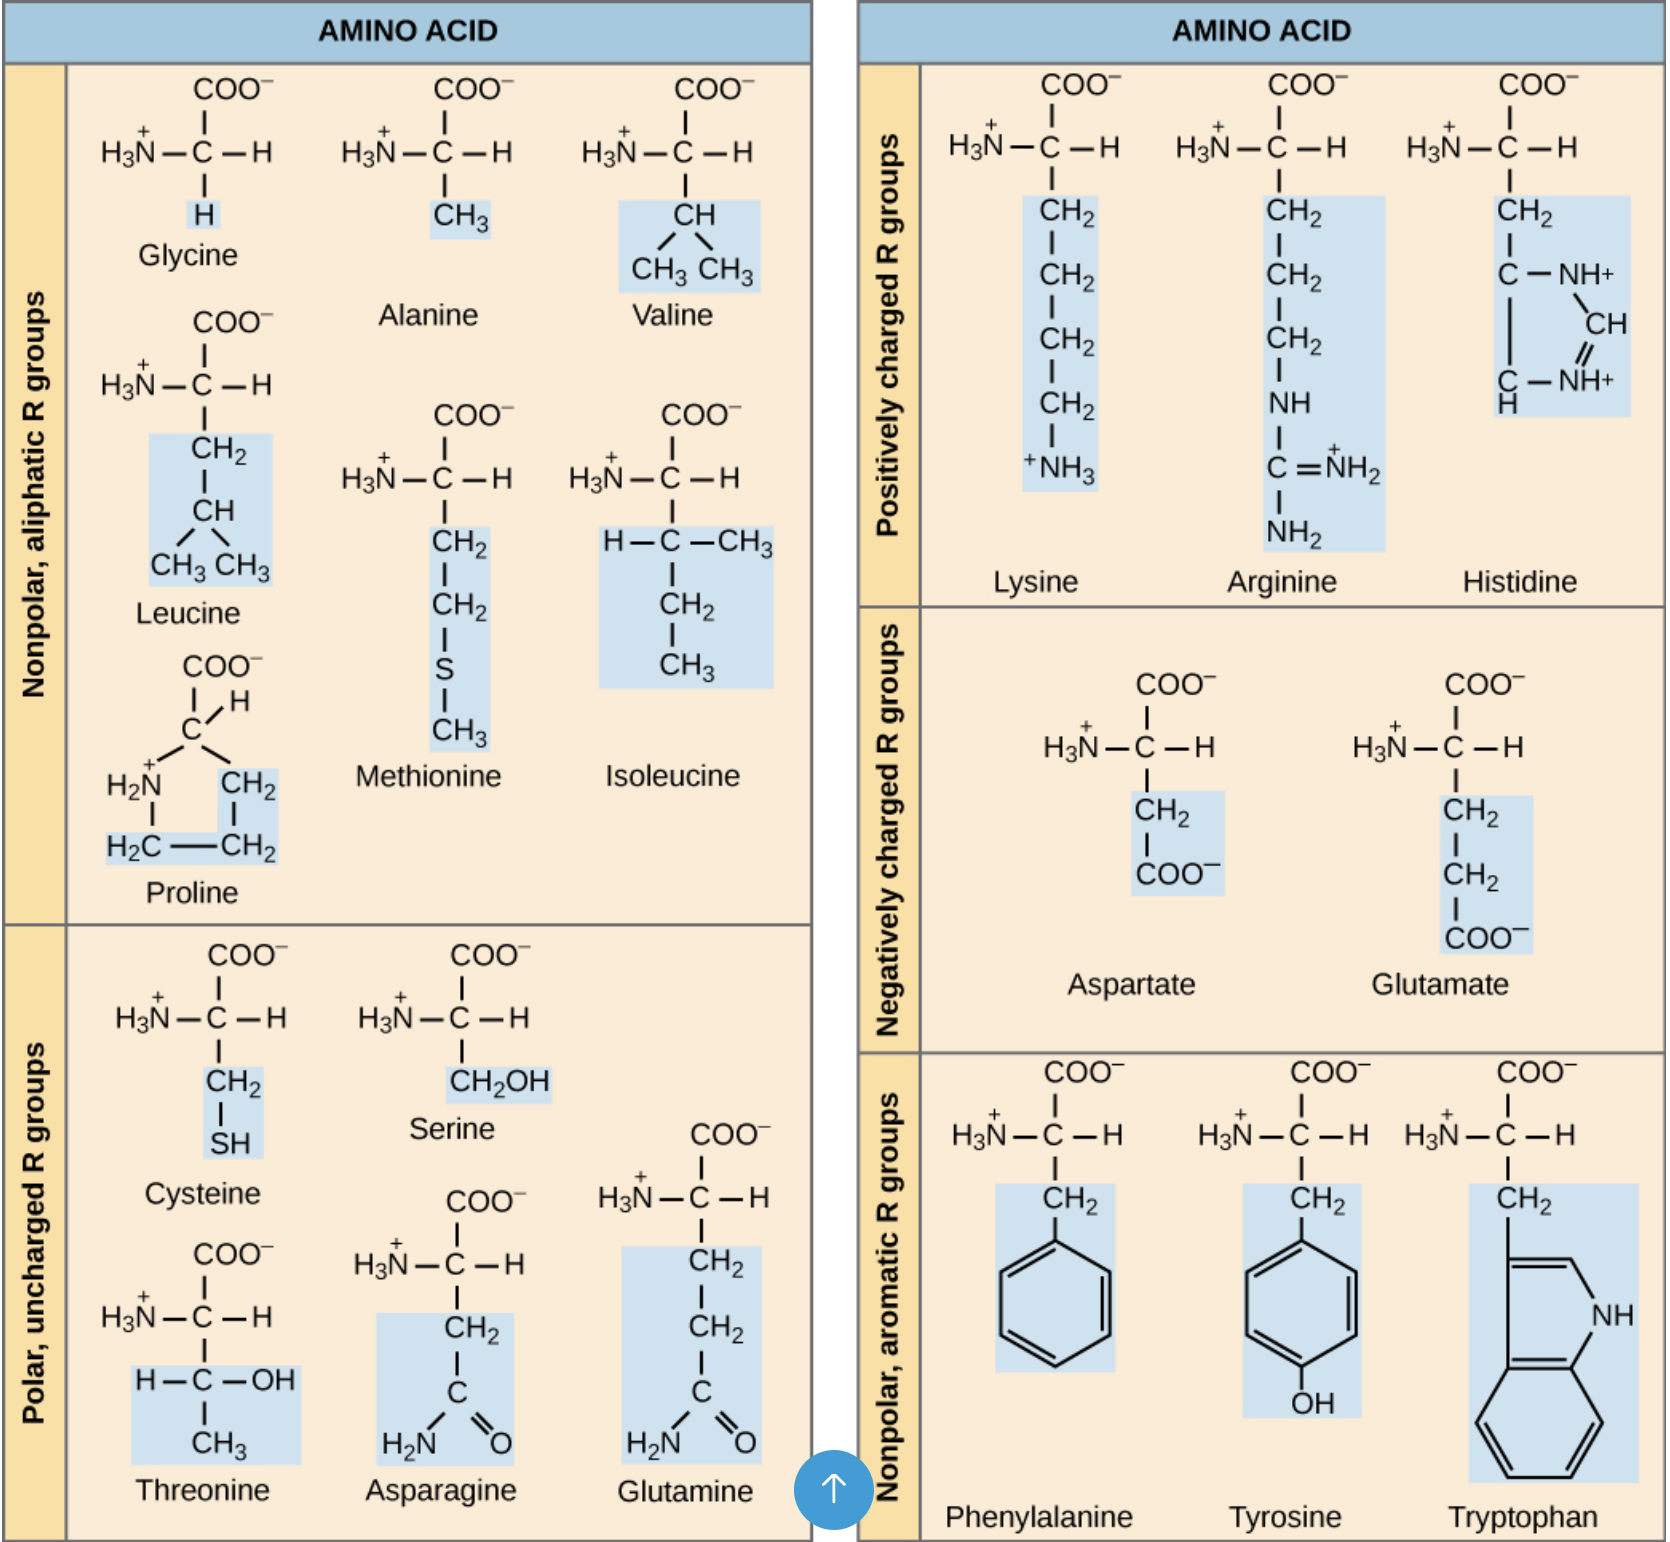
\includegraphics[width=\textwidth]{aas_forreal}
\end{figure}

\subsection*{Spectroscopic properties}

\begin{itemize}
\item No amino acids absorb the visible wavelengths
\item Some residues absorb UV light (W,Y) and are uesd for protein structure determination
\item All amino acids absorb at infrared wavelengths
\item W also exhibits fluorescence
\end{itemize}

\subsection*{Acid base properties}

pH = 1, protonated: both, net charge = +1

pH = 7, protonated: amino group, net charge = 0

pH = 13, protonated: neither, net charge = -1

\textbf{Equivalence point = average of 2 flanking pKas}

\subsection*{The isoelectric point (pI)}
...is the pH at the equivalence point where the molecule has no net charge due to the ionization state of the molecule.

To calculate:

\begin{equation}
pI = \frac{pK_{a \: below} + pK_{a \: above}}{2}
\end{equation}

\newpage

\section*{Peptides}

Amide or peptide bonds link amino acids together in proteins. (amine + carboxyl)

N-terminus at the amino group and C-terminus at the carboxyl group

pKa $>$ pH = positive, pH $<$ pKa = negative

\subsection*{Calculating pI}

\begin{enumerate}
\item What is the charge at neutrality?
\item Arrange all pKa from lowest to highest.
\item Identify neutral form and find flanking pKas.
\item Calculate the average.
\end{enumerate}

Example: Find the pI of this peptide at pH=7:

$$\ce{+H3N}\text{-A-G-R-K-N-I-M-}\ce{COO-}$$

A, G, N, I, M are not ionizable. R and K have a +1 charge. The two ends cancel out.

To find the pI: determine when the net charge = 0.

Deprotonation occurs in this order (by pKa):

\begin{enumerate}
\item C-terminus pKa 2.2
\item N-terminus pKa 9.5
\item K side chain pKa 10.5
\item R side chain pKa 12.5
\end{enumerate}

\end{document}